% Author: Carla Becker, 2026
\documentclass[preprint,12pt]{elsarticle}

% Standard Packages
\usepackage{algorithm}
\usepackage{algorithmicx}
\usepackage{algpseudocode}
\usepackage{amsmath,amssymb,amsfonts}
\usepackage{amsthm}
\usepackage{booktabs}
\usepackage[title]{appendix}
\usepackage{graphicx}
\usepackage{hyperref}
\usepackage{lineno}
\usepackage{listings}
\usepackage{manyfoot}
\usepackage{mathrsfs}
\usepackage{multirow}
\usepackage{textcomp}
\usepackage{xcolor}
\usepackage{colortbl}

% Other
\raggedbottom
\newcommand{\df}[2]{\displaystyle\frac{#1}{#2}}

\journal{Computers and Electronics in Agriculture}

%======================================================================================%
% BEGIN DOCUMENT
%======================================================================================%
\begin{document}
\linenumbers
\begin{frontmatter}
\title{Fixed versus adaptive irrigation and fertilizer management under weather uncertainty: a comparative study using genetic algorithm optimization and model predictive control}

% Author information
\author{Carla J. Becker}
\affiliation{
	organization={Department of Mechanical Engineering, University of California, Berkeley}, % Department and Organization
    addressline={6141 Etcheverry Hall}, 
    city={Berkeley},
    postcode={94720}, 
    state={California},
    country={United States of America}
}

\author{Tarek I. Zohdi}
\affiliation{
	organization={Department of Mechanical Engineering, University of California, Berkeley}, % Department and Organization
    addressline={6141 Etcheverry Hall}, 
    city={Berkeley},
    postcode={94720}, 
    state={California},
    country={United States of America}
}
            	
%======================================================================================%
% ABSTRACT
%======================================================================================%
\begin{abstract}
Climate variability poses significant challenges to agricultural resource management, motivating interest in adaptive control strategies that can respond to observed conditions. This paper tests whether Model Predictive Control (MPC)---an adaptive approach that re-optimizes daily based on current plant state and weather---can outperform fixed strategies optimized via genetic algorithm (GA) for specific conditions. We develop an MPC framework for irrigation and fertilizer scheduling, building on a crop growth model that captures delayed nutrient absorption via finite impulse response (FIR) convolution and cumulative stress tracking via exponential moving average (EMA) filtering. The MPC controller solves a constrained finite-time optimal control (CFTOC) problem at each decision epoch, with Bayesian Optimization using Tree-structured Parzen Estimators (TPE) to tune controller parameters. Evaluated on corn production in Iowa across 21 stochastic weather scenarios, we compare four strategies: farmer best practices (business as usual), GA optimized for normal conditions, GA optimized for drought conditions, and adaptive MPC. We hypothesized that MPC's adaptability would allow it to outperform the fixed GA strategies, but the results do not support this hypothesis. All optimization-based methods outperform farmer best practices (mean revenue \$626/acre), but MPC does not outperform either GA strategy overall. The GA optimized for normal conditions achieves the highest mean revenue (\$842/acre) and lowest coefficient of variation (14.7\%), outperforming MPC (\$750/acre, CV 15.4\%) in all 21 scenarios. The drought-optimized GA (\$796/acre, CV 16.6\%) outperforms the normal-optimized GA only in drought scenarios---an unsurprising result given it was optimized for those conditions. These findings suggest that for seasonal agricultural planning, pre-optimization for expected conditions outperforms adaptive control, and the choice of which GA strategy to use depends simply on whether extreme weather conditions are anticipated. More broadly, optimizing GA strategies for other specific weather conditions (e.g., heat stress, excessive moisture) could similarly achieve better results than a normal-optimized GA when those conditions occur. However, MPC offers a sustainability advantage: it achieves competitive returns while using dramatically less water and fertilizer than all other strategies, which may be valuable where environmental impact or input costs are prioritized.
\end{abstract}


%%Graphical abstract
%\begin{graphicalabstract}
%\includegraphics{grabs}
%\end{graphicalabstract}

%% Research highlights
\begin{highlights}
\item Hypothesis test: can adaptive MPC outperform fixed GA strategies?
\item Four-way comparison across 21 stochastic weather scenarios
\item Result: MPC does not outperform GA strategies; GA (normal) wins all 21 scenarios vs MPC
\item GA (drought) outperforms GA (normal) only in drought scenarios, as expected
\item Conclusion: pre-optimization for expected conditions outperforms adaptive control
\end{highlights}

%% Keywords
\begin{keyword}
precision agriculture \sep
model predictive control \sep
Bayesian optimization \sep
weather uncertainty \sep
adaptive control \sep
\end{keyword}

\end{frontmatter}

%======================================================================================%
% INTRODUCTION
%======================================================================================%
\section{Introduction}\label{sec:intro}

Climate change is increasing the frequency and severity of extreme weather events, posing significant challenges to agricultural production \cite{ipcc2021}. Traditional approaches to irrigation and fertilizer scheduling rely on fixed strategies---either following agronomic best practices or strategies optimized for expected conditions---that cannot adapt when actual weather deviates from assumptions. As drought, heat waves, and other extremes become more common, there is growing interest in adaptive resource management strategies that can respond to observed conditions in real time. Recent work on digital-twin frameworks for precision agriculture \cite{zohdi2024digitaltwin,mengi2023agrivoltaics} and computational approaches to agricultural resource delivery \cite{betancourt2024spray,tagkopoulos2024aifs} have demonstrated the potential for model-based optimization in farming systems.

In a companion paper currently under review \cite{becker2025ga}, we developed a generalized crop growth model based on coupled ordinary differential equations (ODEs) that captures the nonlinear dynamics of plant development under varying environmental conditions. The model tracks five state variables---plant height, leaf area, number of leaves, flower size, and fruit biomass---each governed by logistic growth with time-varying parameters modulated by nutrient factors. These factors quantify how well actual water, fertilizer, temperature, and solar radiation levels match the plant's physiological expectations, with delayed absorption modeled via finite impulse response (FIR) convolution and cumulative stress tracked via exponential moving average (EMA) filtering. Using a genetic algorithm (GA), we showed that optimized irrigation and fertilizer strategies can achieve 16\% higher net revenue than conventional farmer practices under drought conditions.

However, the GA approach optimizes a \emph{fixed} strategy---specifying application frequencies and amounts that remain constant throughout the growing season. While effective when actual conditions match the optimization assumptions, such open-loop strategies cannot adapt to unexpected weather events. If a drought is more severe than anticipated, or an unexpected heat wave occurs, the pre-computed strategy may be far from optimal. This observation motivated the central question of this paper: \emph{can an adaptive control strategy that re-optimizes based on observed conditions outperform a fixed strategy optimized for expected conditions?}

To investigate this question, we develop an adaptive approach using Model Predictive Control (MPC). MPC is a closed-loop control strategy that repeatedly solves an optimization problem over a finite horizon, applies only the first control action, then re-optimizes based on updated state and disturbance information \cite{rawlings2017mpc}. This receding-horizon structure enables the controller to adapt to changing conditions while maintaining optimality over the planning horizon.

Our hypotheses were:
\begin{enumerate}
\item All optimization-based methods (GA and MPC) will outperform farmer best practices (business as usual).
\item MPC's ability to adapt to observed conditions will allow it to outperform fixed GA strategies, particularly in scenarios where weather deviates from the GA's optimization assumptions.
\item A GA optimized for drought conditions will outperform a GA optimized for normal conditions when evaluated across scenarios that include drought.
\end{enumerate}

Applying MPC to agricultural systems presents several challenges. The nonlinear crop dynamics with delayed absorption effects complicate the optimization problem. The controller must balance multiple competing objectives: maximizing crop value, minimizing input costs, and avoiding nutrient stress. The relative importance of these objectives depends on weather conditions and growth stage, requiring careful tuning of the cost function weights. We employ Bayesian Optimization (BO) \cite{shahriari2016taking} with Tree-structured Parzen Estimators (TPE) \cite{bergstra2011algorithms} to automatically tune the MPC parameters for robust performance.

Our contributions are:
\begin{enumerate}
\item Formulation of a constrained finite-time optimal control (CFTOC) problem for daily irrigation and fertilizer scheduling that accounts for delayed nutrient absorption and cumulative stress effects.
\item A receding-horizon MPC implementation with Bayesian-optimized parameters.
\item Systematic comparison of four resource management strategies---farmer best practices, GA optimized for normal conditions, GA optimized for drought conditions, and adaptive MPC---across 21 stochastic weather scenarios spanning from normal to extreme conditions.
\item Empirical evaluation of the hypotheses above, with findings that partially contradict our initial expectations.
\end{enumerate}

Our results support the first hypothesis: all optimization methods outperform farmer best practices. However, the second hypothesis is not supported: MPC does not outperform either GA strategy overall. The GA optimized for normal conditions outperforms MPC in all 21 scenarios. The third hypothesis is also not supported as initially framed: the drought-optimized GA only outperforms the normal-optimized GA in drought scenarios, which is unsurprising given it was specifically optimized for those conditions. These findings suggest that for seasonal agricultural planning, pre-optimization for expected conditions is more effective than adaptive control. We note, however, that this conclusion applies to the specific methods tested here; different MPC formulations (e.g., longer horizons enabled by more computational resources, alternative objective designs, or stochastic MPC that explicitly models forecast uncertainty) might yield different results.


%======================================================================================%
% DYNAMICS
%======================================================================================%
\section{Crop growth model}\label{sec:dynamics}

We employ the crop growth model developed in \cite{becker2025ga}, which we briefly summarize here. The model treats the plant as a dynamic system with state vector $x = [x_{h}, x_{A}, x_{N}, x_{c}, x_{P}]^T$ representing plant height (m), leaf area per leaf (m$^2$), number of leaves, flower size (spikelets), and fruit biomass (kg). Control inputs are irrigation $u_w$ (inches/hour) and fertilizer $u_f$ (lbs/hour), while disturbances include precipitation $d_{S}$ (inches/hour), temperature $d_{T}$ ($^\circ$C), and solar radiation $d_{R}$ (W/m$^2$).

%------------------------------------%
% LOGISTIC GROWTH
%------------------------------------%
\subsection{Logistic growth dynamics}\label{subsec:logistic}

Each state variable follows logistic growth with time-varying parameters:
\begin{equation}
\df{dx}{dt} = \hat{a}_x(t) \cdot x(t) \left(1 - \df{x(t)}{\hat{k}_x(t)}\right)
\label{eqn:logistic}
\end{equation}
where $\hat{a}_x(t)$ is the effective growth rate and $\hat{k}_x(t)$ is the effective carrying capacity, both modulated by nutrient factors. This equation admits a closed-form solution:
\begin{equation}
x(t + \Delta t) = \df{\hat{k}_x(t)}{1 + \left(\df{\hat{k}_x(t)}{x(t)} - 1\right)\exp(-\hat{a}_x(t)\Delta t)}
\label{eqn:closed-form}
\end{equation}
enabling exact time-stepping without numerical integration error.

%------------------------------------%
% DELAYED ABSORPTION
%------------------------------------%
\subsection{Delayed absorption via FIR convolution}\label{subsec:fir}

Plants do not immediately utilize applied nutrients; there is a physiologically-mediated delay between application and absorption. We model this using finite impulse response (FIR) convolution with Gaussian kernels:
\begin{equation}
g[k] = \df{1}{\sqrt{2\pi\sigma^2}}\exp\left\{-\df{(k-\mu)^2}{2\sigma^2}\right\}
\label{eqn:gaussian-kernel}
\end{equation}
where $\sigma$ is the temporal spread characterizing absorption duration. We set $\mu \approx 1.96\sigma$ so that 95\% of the kernel mass lies within $[0, 2\mu]$. Different nutrients have different metabolic timescales: $\sigma_w = 30$ hours for water (rapid uptake), $\sigma_f = 300$ hours for fertilizer (slow root absorption), and $\sigma_T = \sigma_R = 30$ hours for temperature and radiation.

The delayed (absorbed) signal is computed as:
\begin{equation}
\bar{u}[k] = \sum_{n=0}^{L-1} g[n] \cdot u[k-n]
\label{eqn:convolution}
\end{equation}
where $L$ is the FIR horizon chosen to capture 95\% of the kernel mass.

%------------------------------------%
% CUMULATIVE STRESS
%------------------------------------%
\subsection{Cumulative stress tracking}\label{subsec:stress}

While FIR convolution captures delayed absorption, plants also accumulate stress from sustained deviations from optimal conditions. We track cumulative divergence using exponential moving average (EMA) filtering:
\begin{equation}
\Delta_u[k] = \beta_\Delta \cdot \Delta_u[k-1] + (1-\beta_\Delta) \cdot \delta_u[k]
\label{eqn:ema}
\end{equation}
where $\delta_u[k]$ is the instantaneous anomaly (relative deviation from expected cumulative absorption) and $\beta_\Delta = 0.95$ provides long memory of past stress events.

%------------------------------------%
% NUTRIENT FACTORS
%------------------------------------%
\subsection{Nutrient factors}\label{subsec:nutrient-factors}

The cumulative divergence is converted to a nutrient factor $\nu \in [0,1]$ via exponential decay with additional EMA smoothing:
\begin{equation}
\nu_u[k] = \beta_\nu \cdot \nu_u[k-1] + (1-\beta_\nu) \cdot \exp\{-\alpha \Delta_u[k]\}
\label{eqn:nutrient-factor}
\end{equation}
where $\alpha = 3$ ensures $\nu \approx 0.05$ when $\Delta = 1$ (complete divergence). The nutrient factor equals 1 when inputs match expectations and decays toward 0 under sustained stress.

The effective growth parameters are computed as geometric means of relevant nutrient factors. For example, fruit biomass carrying capacity depends on all inputs and prior vegetative growth:
\begin{equation}
\hat{k}_P(t) = k_P \left(\nu_w \nu_f \nu_T \nu_R \df{\hat{k}_h}{k_h} \df{\hat{k}_A}{k_A} \df{\hat{k}_c}{k_c}\right)^{1/7}
\label{eqn:fruit-capacity}
\end{equation}
Full details of the parameter relationships are provided in \cite{becker2025ga}.


%======================================================================================%
% STOCHASTIC WEATHER
%======================================================================================%
\section{Stochastic weather scenario generation}\label{sec:weather}

To evaluate controller robustness, we generate a suite of stochastic weather scenarios from historical baseline data. Each scenario applies perturbations representing different climate conditions, from normal variability to extreme events. A single scenario can comprise multiple weather events. In this study, the possible types of weather events are droughts/downpours $\mathcal{D}$ and heat waves/cold snaps $\mathcal{H}$. The process of adding perturbations to the historical baseline data in order to obtain synthetic, stochastic, and at times extreme, weather data is as follows: 1) scale the precipitation and radiation data by fixed scaling factors, offset the temperature data by a fixed value, 2) add white noise to each time step, independent from other time steps, 3) apply all events of type $\mathcal{D}$, 4) apply all events of type $\mathcal{H}$, and 5) check that synthetic data falls within reasonable physical bounds. Details of those transformations follow below.

%------------------------------------%
% WEATHER GENERATION PROCESS
%------------------------------------%
\subsection{Generation process}\label{subsec:weather-generation}

Let the historical hourly time series be
\begin{gather}
d_{S}^{\text{hist}}[k] \geq 0           \\
-20 \leq d_{T}^{\text{hist}}[k] \leq 50 \\
d_{R}^{\text{hist}}[k] \geq 0
\label{eqn:history}
\end{gather}
for $k=0,...,K-1$ where $K$ is the length of the growing season in hours, respectively representing precipitation (inches), temperature (\textdegree C), and solar radiation (W/m\textsuperscript{2}). Then, let a stochastic weather scenario be defined by the parameters
\begin{equation}
\theta = (s_{S}, s_{T}, s_{R}, \eta, \mathcal{D}, \mathcal{H})
\label{eqn:weather-scenario}
\end{equation}
where
\begin{itemize}
\item $s_{S} \in [0, 2]$ is the precipitation adjustment (scaling factor)
\item $s_{T} \in \mathbb{R}$ is the temperature adjustment (offset)
\item $s_{R} \in [0, 2]$ is the radiation adjustment (scaling factor)
\item $\eta \in [0, 1]$ is the relative noise level (a fraction of the historical standard deviation)
\item $\mathcal{D}$ is a drought or downpour event
\item $\mathcal{H}$ is a heat wave or cold snap event
\end{itemize}

Each event types is defined by three parameters:
\begin{equation}
[k_{0}, \kappa, \iota]
\label{eqn:event}
\end{equation}
where
\begin{itemize}
\item $k_{0}$ is the hour when the event begins
\item $\kappa$ is the duration of the event in number of hours
\item $\iota\in[0,1]$ is the intensity, with 1 being the most intense
\end{itemize}

% STEP 1: Global scaling and offset
\subsubsection{Global scaling and offset}\label{subsubsec:weather-step-1}

Initialize the synthetic environmental disturbance time series by applying the global adjustments $(s_{S}, s_{T}, s_{R})$ for $k=0,...,K-1$ as below
\begin{equation}
\begin{array}{ll}
d_{S}^{(1)}[k] = s_{S}d_{S}^{\text{hist}}[k]    & \text{(scaling)} \\[7pt]
d_{T}^{(1)}[k] = d_{T}^{\text{hist}}[k] + s_{T} & \text{(offset)}  \\[7pt]
d_{R}^{(1)}[k] = s_{R}d_{R}^{\text{hist}}[k]    & \text{(scaling)}
\end{array}
\label{eqn:global-scaling}
\end{equation}

% STEP 2: Add white noise
\subsubsection{Add white noise}\label{subsubsec:weather-step-2}

If $\eta > 0$, draw independent white noise sequences
\begin{align}
\varepsilon_{T}[k] \sim \mathcal{N}(0, (\eta\sigma_{T})^{2}) \\
\varepsilon_{R}[k] \sim \mathcal{N}(0, (\eta\sigma_{R})^{2})
\label{eqn:varepsilon}
\end{align}
where $\sigma_{T}$ and $\sigma_{R}$ are the standard deviations of the historical temperature and radiation time series, respectively.

We then smooth the white noise with a moving average over $m_{T} = 24$ hours for temperature and $m_{R} = 12$ hours for radiation, as we will only apply the noise to the radiation during the day time (when it is not as close to zero).
\begin{align}
\bar{\varepsilon}_{T}[k] = \df{1}{m_{T}} \sum_{n=0}^{m_{T} - 1} \varepsilon_{T}[k-n] \\
\bar{\varepsilon}_{R}[k] = \df{1}{m_{R}} \sum_{n=0}^{m_{R} - 1} \varepsilon_{R}[k-n]
\label{eqn:smooth-noise}
\end{align}
The smoothed noise is then added to the signals from section \ref{subsubsec:weather-step-1}.
\begin{align}
d_{T}^{(2)}[k] = d_{T}^{(1)}[k] + \bar{\varepsilon}_{T}[k] \\
d_{R}^{(2)}[k] = d_{R}^{(1)}[k] + \mathcal{M}_{\text{day}}\bar{\varepsilon}_{R}[k]
\label{eqn:add-noise}
\end{align}
where
\begin{equation}
\mathcal{M}_{\text{day}} = \{ k | d_{R}^{\text{hist}}[k] > d_{R}^{\text{day}} \}
\label{eqn:daymask}
\end{equation}
and we choose the threshold $d_{R}^{\text{day}} = 10$ W/m\textsuperscript{2}. Precipitation is unchanged in this step, so
\begin{equation}
d_{S}^{(2)}[k] = d_{S}^{(1)}[k]
\label{eqn:P2-P1}
\end{equation}
If $\eta = 0$, then we let $(d_{S}^{(2)}, d_{T}^{(2)}, d_{R}^{(2)}) = (d_{S}^{(1)}, d_{T}^{(1)}, d_{R}^{(1)})$.

% STEP 3: Drought Injection
\subsubsection{Drought/downpour injection}\label{subsubsec:drought-injection}

A drought or downpour event is
\begin{equation}
\mathcal{D} = [k_{0}, \kappa, \iota]
\label{eqn:drought-event}
\end{equation}

and drought events only affect synthetic precipitation. Each event takes place for a limited amount of time, so only some time steps are affected. For each event, we define the affected hourly index set as
\begin{equation}
\mathcal{I} = \{ k_{0}, k_{0}+1,...,\min(k_{0} + \kappa - 1, K-1) \},
\label{eqn:affected-indices}
\end{equation}
so either $\kappa$ steps or the end of the season, whichever comes first, and then apply the intensity scaling to those indices with
\begin{equation}
d_{S}^{(3)}[k] \leftarrow (1 - \iota)d_{S}^{(2)}[k] \quad \text{for all } k\in\mathcal{I}
\label{eqn:P3}
\end{equation}
Temperature and radiation are unchanged in this step, so
\begin{equation}
d_{T}^{(3)}[k] = d_{T}^{(2)}[k] \quad \text{and} \quad d_{R}^{(3)}[k] = d_{R}^{(2)}[k]
\label{eqn:T3R3-T2R2}
\end{equation}

% STEP 4: Heat Wave Injection
\subsubsection{Heat wave/cold snap injection}\label{subsubsec:heat-wave-injection}

A heat wave or cold snap event affects only synthetic temperature and is defined by
\begin{equation}
\mathcal{H} = [k_{0}, \kappa, \iota]
\label{eqn:heatwave-event}
\end{equation}
where $k_{0}$ and $\kappa$ have the same meanings they did for the drought event, but now $\iota$ is the peak/valley temperature difference (an offset rather than a scaling factor). We then construct a ramp-up, hold, and ramp-down for the event. Let
\begin{equation}
\kappa_{\text{ramp}} = \max(1, 0.1\kappa)
\label{eqn:kappa-ramp}
\end{equation}
i.e. either one tenth of the heat wave duration or at least one hour. Then, let
\begin{equation}
\kappa_{\text{hold}} = \kappa - 2\kappa_{\text{ramp}}
\label{eqn:kappa-hold}
\end{equation}
to account for the ramp-up and ramp-down.

We can then define
\begin{itemize}
\item ramp-up:   $w_{\text{up}}[k]   = \df{k}{\kappa_{\text{ramp}} - 1}$ for $k=0,...,\kappa_{\text{ramp}} - 1$
\item ramp-hold: $w_{\text{hold}}[k] = 1$
\item ramp-down: $w_{\text{down}}[k] = \df{k}{\kappa_{\text{ramp}} - 1}$ for $k=0,...,\kappa_{\text{ramp}} - 1$
\end{itemize}
and concatenate to form the heat wave window
\begin{equation}
w_{\text{heat}} = [w_{\text{up}}, w_{\text{hold}}, w_{\text{down}}]
\label{eqn:w-heat}
\end{equation}
Applying the event to the temperature time series, we obtain
\begin{equation}
d_{T}^{(4)}[k] \leftarrow d_{T}^{(3)}[k] \pm \iota w_{\text{heat}}[k - k_{0}]
\label{eqn:T4a}
\end{equation}
for $k=k_{0}, k_{0}+1,...,\min(k_{0}+ \kappa - 1, K-1)$, where $\iota$ is added in the case of a heat wave and subtracted in the case of a cold snap. Precipitation and radiation are unchanged in this step, so
\begin{equation}
d_{S}^{(4)}[k] = d_{S}^{(3)}[k] \quad \text{and} \quad d_{R}^{(4)}[k] = d_{R}^{(3)}[k]
\label{eqn:P4P3-R4R3}
\end{equation}

% STEP 5: Clipping to Physical Bounds
\subsubsection{Clipping to physical bounds}\label{subsubsec:clipping}

Finally, we check to ensure that the transformations above have not violated the bounds on the input disturbances specified in equations \ref{eqn:history}. If they have, we clip the values as below
\begin{align}
d_{S}^{\text{syn}}[k] &= \max(0, d_{S}^{(4)}[k]) \\
d_{T}^{\text{syn}}[k] &= \min(50, \max(-20, d_{T}^{(4)}[k])) \\
d_{R}^{\text{syn}}[k] &= \max(0, d_{R}^{(4)}[k])
\label{eqn:PTR-syn}
\end{align}
for all $k\in\{ 0,...,K-1 \}$.

%------------------------------------%
% EXTREMITY INDEX
%------------------------------------%
\subsection{Extremity index}\label{subsec:extremity}

To systematically compare strategy performance across diverse conditions, we define an extremity index $\mathcal{E}$ that quantifies how far a scenario deviates from baseline conditions. This index serves two purposes: (1) analyzing whether different optimization methods perform better at different extremity levels, and (2) ensuring that MPC parameter tuning covers a representative range of conditions. The index aggregates contributions from precipitation anomalies, temperature anomalies, and discrete weather events, with each component normalized so that a value of 1 represents a meaningful agronomic threshold---i.e., a deviation large enough to require management intervention or cause measurable yield impact.

\noindent\textbf{Precipitation extremity.} The precipitation scaling factor $s_S$ determines seasonal water availability, with $s_S = 1$ representing baseline conditions. Deviations in either direction---drought ($s_S < 1$) or excess moisture ($s_S > 1$)---contribute to extremity:
\begin{equation}
\mathcal{E}_{\text{precip}} = 2|1 - s_{S}|
\label{eqn:extreme-precip}
\end{equation}
The factor of 2 is chosen so that a 50\% reduction in precipitation ($s_S = 0.5$) yields $\mathcal{E}_{\text{precip}} = 1$. This threshold reflects agronomic practice: a 50\% precipitation deficit during the growing season typically triggers supplemental irrigation and is considered a moderate drought requiring active management \cite{kranz2008irrigation}.

\noindent\textbf{Temperature extremity.} Seasonal temperature offsets contribute to extremity based on their magnitude:
\begin{equation}
\mathcal{E}_{\text{temp}} = \df{|s_{T}|}{5}
\label{eqn:extreme-temp}
\end{equation}
The $\pm 5$\textdegree C threshold reflects corn physiology: sustained temperatures above 35\textdegree C or below 10\textdegree C significantly reduce photosynthesis and pollen viability \cite{hatfield2015temperature}. Since mean baseline temperature is approximately 23\textdegree C, a 5\textdegree C offset moves conditions into ranges where yield impacts become measurable.

\noindent\textbf{Drought event extremity.} Discrete drought events contribute based on their duration and intensity:
\begin{equation}
\mathcal{E}_{\text{drought}} = \sum_{(k_{0}, \kappa, \iota)\in\mathcal{D}} \df{\kappa}{500}\iota
\label{eqn:extreme-drought}
\end{equation}
The 500-hour (approximately 21-day) normalization reflects the timescale over which soil moisture depletion becomes critical. Corn can typically tolerate 7--10 days without rainfall before showing stress symptoms; by three weeks, yield losses become significant without irrigation intervention \cite{kranz2008irrigation}. A full-intensity drought lasting 21 days thus represents the threshold for serious crop impact.

\noindent\textbf{Heat wave and cold snap extremity.} Temperature events contribute based on both duration and intensity:
\begin{equation}
\mathcal{E}_{\text{heat}} = \sum_{(k_{0}, \kappa, \iota)\in\mathcal{H}} \df{\kappa}{200}\df{\iota}{5}
\label{eqn:extreme-heatwave}
\end{equation}
The 200-hour (approximately 8-day) duration threshold reflects the timescale over which sustained heat stress affects corn reproductive development. During tasseling and silking, even brief heat waves can reduce kernel set, but cumulative effects become severe after about one week \cite{hatfield2015temperature}. The 5\textdegree C intensity threshold again corresponds to the deviation that moves temperatures into physiologically stressful ranges.

\noindent\textbf{Aggregate extremity.} The total extremity index is the sum of all components:
\begin{equation}
\mathcal{E} = \mathcal{E}_{\text{precip}} + \mathcal{E}_{\text{temp}} + \mathcal{E}_{\text{drought}} + \mathcal{E}_{\text{heat}}
\label{eqn:extremity}
\end{equation}

%======================================================================================%
% MPC
%======================================================================================%
\section{Model predictive control}\label{sec:mpc}

%------------------------------------%
% Intro to Optimization
%------------------------------------%
\subsection{Optimization and decision epochs}\label{subsec:optimization}

Model Predictive Control frames resource allocation as a sequence of optimization problems. At each \emph{decision epoch}---in our case, the start of each day---the controller observes the current system state and solves an optimization problem to determine the best actions over a finite planning horizon. The solution specifies how much irrigation and fertilizer to apply, balancing immediate costs against long-term crop development.

This approach differs fundamentally from the genetic algorithm method used in our companion paper \cite{becker2025ga}, which optimizes a single fixed strategy over the entire growing season. MPC instead solves a smaller optimization problem at each decision epoch, using updated state and forecast information to adapt to changing conditions.

%------------------------------------%
% CFTOC
%------------------------------------%
\subsection{Constrained finite-time optimal control}\label{subsec:cftoc}

At each decision epoch, model predictive control (MPC) solves a constrained finite-time optimal control (CFTOC) problem over a planning horizon of $K_{d}$ days. Discrete-time optimal control is concerned with choosing an optimal input sequence over the horizon $K_{d}$
\begin{equation}
\mathcal{U}_{0\to K_{d}} = \{ u[k] \} \quad \text{for} \quad k=0,...,K_{d}-1
\label{eqn:U0K}
\end{equation}
with respect to some objective function over a finite or infinite time horizon in order to apply it to a system with a given initial state $x[0]$. The objective function is often defined as a sum of stage costs $q(x[k], u[k])$ and when the horizon has finite length, a terminal cost $p(x[K_{d}])$. That is
\begin{equation}
J_{0\to K_{d}}(x[0], \mathcal{U}_{0\to K_{d}}) = p(x[K_{d}]) + \sum_{n=0}^{K_{d}-1} q(x[n], u[n])
\label{eqn:gen-opt-ctrl-cost}
\end{equation}
where the states $\mathcal{X}_{0\to K_{d}} = \{ x[k] \} \quad \text{for} \quad k=0,...,K_{d}-1$ must satisfy the initial condition and system dynamics
\begin{equation}
\begin{cases}
x[0] = x_{0} \\
x[k+1] = g(x[k], u[k]) & \text{for } k=0,...,K_{d}-1
\end{cases}
\label{eqn:dyn-constraint}
\end{equation}
and there may be other state or input constraints formulated as inequalities
\begin{equation}
h(x[k], u[k]) \leq 0 \quad \text{for} \quad k=0,...,K_{d}-1
\label{eqn:ineq-constraints}
\end{equation}
In the finite horizon case, there may also be a terminal constraint requiring the final state to lie in some terminal set $x[K]\in\mathcal{X}_{\text{final}}$.

In our specific case, we construct the problem as a minimization
\begin{equation}
\begin{array}{c}
J_{0\to K_{d}}^{*}(x[0]) = \min\limits_{\mathcal{U}_{0\to K_{d}}} J_{0\to K_{d}}(x[0], \mathcal{U}_{0\to K_{d}}) \quad \text{s.t.} \\[7pt]
\begin{cases}
x[0] = x_{0} \\
x[k+1] = g(x[k], u[k]) & \text{for } k=0,...,K_{d}-1 \\
x\in\mathbb{R}^{+} \\
u\in{\mathcal{U}}
\end{cases}
\end{array}
\label{eqn:minimization-cftoc}
\end{equation}
where the stage cost penalizes input usage and nutrient anomalies:
\begin{equation}
q(x[k], u[k]) =
\underbrace{\omega_{w}\left( \df{u_{w}[k]}{u_{w,\text{typ}}} \right)^{2} +
\omega_{f}\left( \df{u_{f}[k]}{u_{f,\text{typ}}} \right)^{2}}_{\text{input usage}} +
\underbrace{\omega_{\Delta w}(\Delta_{w}[k])^{2} +
\omega_{\Delta f}(\Delta_{f}[k])^{2}}_{\text{nutrient anomalies}}
\label{eqn:stage-cost}
\end{equation}
Here $\omega_w$ and $\omega_f$ are weights on normalized irrigation and fertilizer inputs, $u_{w,\text{typ}}$ and $u_{f,\text{typ}}$ are typical application rates, and $\omega_{\Delta w}$ and $\omega_{\Delta f}$ penalize the cumulative nutrient anomalies $\Delta_w$ and $\Delta_f$ defined in (\ref{eqn:ema}). The terms in the stage cost have been squared in order to encourage sparsity in actuation, more similar to what a farmer might actually implement. 

The terminal cost rewards crop development:
\begin{equation}
p(x[K_{d}]) =
-\omega_{h}\df{x_{h}[K_{d}]}{k_{h}} -
\omega_{A}\df{x_{A}[K_{d}]}{k_{A}} -
\omega_{P}\df{x_{P}[K_{d}]}{k_{P}}
\label{eqn:terminal-cost}
\end{equation}
where $\omega_h$, $\omega_A$, and $\omega_P$ weight the normalized final height, leaf area, and fruit biomass, respectively, and we treat a reward as a negative cost. There is no terminal set constraint because we want the plant to grow as much as possible. 

%------------------------------------%
% SOLUTION METHOD
%------------------------------------%
\subsection{Solution method}\label{subsec:solution}

The CFTOC problem is formulated in Pyomo \cite{bynum2021pyomo} and solved using the IPOPT interior-point nonlinear optimizer \cite{wachter2006ipopt} with the MUMPS linear solver. The nonlinearity arises from the logistic dynamics, FIR convolution, EMA filtering, and exponential nutrient factor computation.

%------------------------------------%
% ALGORITHM
%------------------------------------%
\subsection{Receding-horizon algorithm}\label{subsec:mpc-algorithm}

MPC implements the CFTOC in a receding-horizon fashion, re-optimizing daily based on updated state and weather observations. Let $k$ index the decision day, and let $u[k] = (u_{w}[k], u_{f}[k])$ denote the daily irrigation and fertilizer rates. Let $\hat{d_{S}}, \hat{d_{T}}, \hat{d_{R}}$ denote forecast weather and $d_S, d_T, d_R$ denote actual observed weather (precipitation, temperature, radiation).

Algorithm \ref{alg:mpc} presents the MPC procedure. At each decision day $k$:
\begin{enumerate}
\item Observe current plant state $x[k]$ and obtain $K_{d}$-day weather forecast $\{(\hat{d_{S}}, \hat{d_{T}}, \hat{d_{R}})_{k+i}\}_{i=0}^{K_{d}-1}$.
\item Solve the CFTOC problem (\ref{eqn:minimization-cftoc}) to obtain optimal control sequence $\{u^*[k+j]\}_{i=0}^{K_{d}-1}$.
\item Apply only the first control $u^*[k] = (u_{w}[k], u_{f}[k])$ uniformly over day $k$.
\item Simulate hourly plant dynamics over the day using actual (not forecast) weather.
\item Advance to day $k+1$ and repeat.
\end{enumerate}

\begin{algorithm}[ht]
\caption{Model Predictive Control for Irrigation and Fertilization}
\label{alg:mpc}
\begin{algorithmic}[1]
\State \textbf{Input:} Initial state $x[0]$, horizon $K_{d}$, season length $K$ days, weather data
\State \textbf{Output:} Control history $\{u[k]\}_{k=0}^{K-1}$, final state $x[K]$
\State
\State Initialize FIR kernel buffers, EMA state variables
\For{$k = 0$ to $K-1$}
    \State Aggregate hourly weather forecast into daily averages for days $k, \ldots, k+K_{d}-1$
    \State Solve CFTOC$(x[k], \{(\hat{d_{S}}, \hat{d_{T}}, \hat{d_{R}})_{k+i}\}_{i=0}^{K_{d}-1})$ $\rightarrow$ $\{u^*[k+i]\}_{i=0}^{K_{d}-1}$
    \State Extract first control: $(u_{w}[k], u_{f}[k]) \leftarrow u^*[k]$
    \For{$t = 0$ to $23$} \Comment{Hourly simulation within day $k$}
        \State Apply $(u_{w}[k]/24, u_{f}[k]/24)$ with actual weather $(d_{S, 24k+t}, d_{T, 24k+t}, d_{R, 24k+t})$
        \State Update FIR buffers, EMA states, nutrient factors
        \State Advance plant state using closed-form logistic solution (\ref{eqn:closed-form})
    \EndFor
    \State $x_{k+1} \leftarrow$ current plant state
\EndFor
\State \Return $\{u[k]\}_{k=0}^{K-1}$, $x[K_{d}]$
\end{algorithmic}
\end{algorithm}

%------------------------------------%
% FEEDBACK PROPERTIES
%------------------------------------%
\subsection{Feedback properties}\label{subsec:feedback}

In theory, the key advantage of MPC over open-loop optimization (such as GA) is its closed-loop nature. By re-solving the optimization problem each day with updated state and weather information, MPC can:
\begin{itemize}
\item \textbf{Correct for forecast errors:} If yesterday's weather differed from the forecast, today's optimization accounts for the actual plant state.
\item \textbf{Adapt to changing conditions:} If a heat wave arrives unexpectedly, MPC can adjust irrigation to maintain nutrient factors.
\item \textbf{Exploit updated forecasts:} Longer-range forecasts become more accurate as the event approaches.
\end{itemize}


%======================================================================================%
% BAYESIAN OPTIMIZATION
%======================================================================================%
\section{Bayesian optimization for MPC parameter tuning}\label{sec:bo}

The MPC cost function contains seven tunable weights: $\omega_w, \omega_f, \omega_{\Delta w}, \omega_{\Delta f}, \omega_h, \omega_A, \omega_P$, plus the horizon length $K_{d}$. These parameters significantly affect controller behavior, and their optimal values depend on the weather scenario ensemble. We use Bayesian Optimization (BO) to automatically tune these parameters for robust performance.

%------------------------------------%
% BO OVERVIEW
%------------------------------------%
\subsection{Bayesian optimization and tree-structured Parzen estimators}\label{subsec:bo-overview}

Bayesian Optimization (BO) is well-suited to hyperparameter tuning problems where function evaluations are expensive and gradients are unavailable \cite{shahriari2016taking}. The approach maintains a probabilistic model of the objective function and uses this model to decide where to sample next, balancing exploration of uncertain regions against exploitation of promising regions.

Tree-structured Parzen Estimation (TPE) \cite{bergstra2011algorithms} models $p(x|y)$ rather than $p(y|x)$ directly, using two density functions. Observations are partitioned by a quantile threshold $\gamma$ (typically 0.1--0.25) into ``good'' and ``bad'' sets, with corresponding densities $l(x) = p(x|y\leq y^{-})$ and $g(x) = p(x|y > y^{-})$, where $y^{-}$ is the $\gamma$-quantile of observed values. Starting from expected improvement and applying Bayes' rule, one can show that maximizing expected improvement is equivalent to maximizing $l(x)/g(x)$, which serves as the TPE acquisition function.

TPE approximates the densities $l(x)$ and $g(x)$ using kernel density estimation (KDE), placing Gaussian kernels around observed data points. For multivariate parameters, TPE assumes independence across dimensions, and the ``tree-structured'' aspect accommodates conditional parameter dependencies. TPE offers computational advantages over GP-based methods and handles mixed parameter spaces (continuous, discrete, categorical)---properties that make it well-suited for MPC parameter tuning, where the objective landscape may contain discontinuities from solver failures and the search space includes both continuous weights and integer horizon length.

%------------------------------------%
% SEARCH SPACE
%------------------------------------%
\subsection{Search space}\label{subsec:search-space}

Table \ref{tab:search-space} defines the search space for MPC parameter tuning. Stage cost weights use log-scale sampling to span multiple orders of magnitude, terminal cost weights use linear sampling (as ask prices for the crop do not fluctuate over multiple magnitudes), and integer sampling is used for the horizon.

\begin{table}[ht]
\centering
\begin{tabular}{|c|c|c|c|}
\hline
Parameter & Lower & Upper & Scale \\
\hline\hline
$\omega_w$          (irrigation cost)     & 0.001  & 10.0    & log     \\
$\omega_f$          (fertilizer cost)     & 0.0001 & 1.0     & log     \\
$\omega_{\Delta w}$ (water anomaly)       & 0.001  & 10.0    & log     \\
$\omega_{\Delta f}$ (fertilizer anomaly)  & 0.001  & 10.0    & log     \\
$\omega_h$          (height value)        & 10.0   & 1000.0  & linear  \\
$\omega_A$          (leaf area value)     & 10.0   & 1000.0  & linear  \\
$\omega_P$          (fruit biomass value) & 100.0  & 10000.0 & linear  \\
$H$                 (horizon, days)       & 3      & 14      & integer \\
\hline
\end{tabular}
\caption{Bayesian optimization search space for MPC parameters.}
\label{tab:search-space}
\end{table}


%------------------------------------%
% ROBUST OPTIMIZATION
%------------------------------------%
\subsection{Robust optimization objective}\label{subsec:robust-objective}

For robust parameter tuning, we optimize average performance across multiple weather scenarios:
\begin{equation}
\boldsymbol{\theta}^* = \arg\max_{\boldsymbol{\theta}} \df{1}{|\mathcal{S}|} \sum_{\mathcal{S}_i \in \mathcal{S}} \text{Revenue}(\text{MPC}(\boldsymbol{\theta}, \mathcal{S}_i))
\label{eqn:robust-objective}
\end{equation}
where $\mathcal{S}$ is a representative subset of weather scenarios and $\boldsymbol{\theta} \in \boldsymbol{\Theta}$, the hyperrectangular search space defined in Table~\ref{tab:search-space}. This encourages parameters that perform well across diverse conditions rather than overfitting to a single scenario.

%------------------------------------%
% ALGORITHM
%------------------------------------%
\subsection{TPE algorithm}\label{subsec:bo-algorithm}

Algorithm~\ref{alg:bo} presents the TPE-based parameter tuning procedure. The objective function averages MPC performance across multiple weather scenarios, encouraging parameters that perform well across diverse conditions rather than overfitting to a single scenario.

\begin{algorithm}[ht]
\caption{Bayesian Optimization for MPC Parameter Tuning}
\label{alg:bo}
\begin{algorithmic}[1]
\State \textbf{Input:} Search space $\boldsymbol{\Theta}$ (Table \ref{tab:search-space}), weather scenarios $\mathcal{S}$, budget $N$, startup trials $N_0$
\State \textbf{Output:} Optimal parameters $\boldsymbol{\theta}^*$
\State
\State Initialize TPE surrogate model
\For{$n = 1$ to $N$}
    \If{$n \leq N_0$}
        \State $\boldsymbol{\theta}_n \leftarrow$ sample uniformly from $\boldsymbol{\Theta}$
    \Else
        \State $\boldsymbol{\theta}_n \leftarrow \arg\max_{\boldsymbol{\theta}} \mathbb{E}(\boldsymbol{\theta})$ using TPE
    \EndIf
    \State
    \State $r_n \leftarrow 0$
    \For{each scenario $\mathcal{S}_i \in \mathcal{S}$}
        \State Run MPC with parameters $\boldsymbol{\theta}_n$ on scenario $\mathcal{S}_i$
        \State $r_n \leftarrow r_n + \text{Revenue}_i / |\mathcal{S}|$
    \EndFor
    \State Update TPE model with observation $(\boldsymbol{\theta}_n, r_n)$
\EndFor
\State
\State $\boldsymbol{\theta}^* \leftarrow \arg\max_n r_n$
\State \Return $\boldsymbol{\theta}^*$
\end{algorithmic}
\end{algorithm}

We use $N = 100$ trials with $N_0 = 20$ random startup trials before engaging the TPE sampler. For robust optimization, we use a representative subset of 5 scenarios spanning the extremity range.


%======================================================================================%
% CASE STUDY
%======================================================================================%
\pagebreak
\section{Case study: corn in Iowa}\label{sec:case-study}

We demonstrate the framework using corn, the most widely planted crop in the United States with over 90 million acres harvested annually \cite{fsa-acreage}. The case study uses historical weather data from Fairfax, Iowa (41.76$^{\circ}$N, 91.87$^{\circ}$W), a representative location in the Corn Belt (USDA climate zones 4b--5b).

%------------------------------------%
% SCENARIO SETUP
%------------------------------------%
\subsection{Scenario configuration}\label{subsec:scenario}

The simulation covers a typical growing season from late April to early October (approximately 2900 hours). Environmental inputs are:

\begin{itemize}
\item \textbf{Temperature and radiation:} Hourly data from NSRDB for Fairfax, IA. Mean temperature is 22.8$^{\circ}$C; mean solar radiation is 580 W/m$^{2}$.
\item \textbf{Precipitation:} Daily data from NOAA, interpolated to hourly resolution.
\item \textbf{Typical nutrient expectations:} Based on agronomic recommendations \cite{corn-nutrient-management}, the model expects 28 inches of water and 355 lbs of NPK fertilizer over the season ($w_{\text{typ}} \approx 0.01$ in/hr, $f_{\text{typ}} \approx 0.12$ lb/hr).
\end{itemize}

%------------------------------------%
% FOUR STRATEGIES
%------------------------------------%
\subsection{Four strategies for comparison}\label{subsec:strategies}

We compare four irrigation and fertilization strategies representing different approaches to resource management:

\textbf{Farmer Best Practices.} Standard agronomic best practices based on published recommendations \cite{kranz2008irrigation,davies2020nitrogen}: weekly irrigation at 1 inch per application, and monthly fertilization at 90 lbs per application. This represents what a well-informed farmer might implement without optimization.

\textbf{GA (Drought).} A strategy optimized via genetic algorithm \cite{becker2025ga} for drought conditions (50\% of historical precipitation). The GA searches over four parameters---irrigation frequency, irrigation amount, fertilizer frequency, and fertilizer amount---to maximize net revenue. The optimal strategy applies irrigation every 52 days at 5.0 inches per application, and fertilizer every 33 days at 77 lbs per application.

\textbf{GA (Normal).} A strategy optimized via genetic algorithm for normal weather conditions (100\% of historical precipitation). The optimal strategy applies irrigation every 81 days at 2.1 inches per application, and fertilizer every 9 days at 30 lbs per application. Compared to GA (Drought), this strategy uses less irrigation per application but applies fertilizer more frequently in smaller doses.

\textbf{Adaptive MPC.} Model Predictive Control that re-optimizes daily based on observed weather and current plant state. Unlike the fixed strategies, MPC adjusts resource allocation throughout the growing season in response to actual conditions.

Table~\ref{tab:strategy-params} summarizes the control parameters for each strategy.

\begin{table}[ht]
\centering
\begin{tabular}{|l|c|c|c|c|}
\hline
Strategy & \begin{tabular}[c]{@{}c@{}}Irrig. Freq.\\(days)\end{tabular} & \begin{tabular}[c]{@{}c@{}}Irrig. Amt.\\(in)\end{tabular} & \begin{tabular}[c]{@{}c@{}}Fert. Freq.\\(days)\end{tabular} & \begin{tabular}[c]{@{}c@{}}Fert. Amt.\\(lbs)\end{tabular} \\
\hline\hline
Farmer Best Practices & 7             & 1.0      & 30            & 90       \\
GA (Drought)          & 52            & 5.0      & 33            & 77       \\
GA (Normal)           & 81            & 2.1      & 9             & 30       \\
Adaptive MPC          & Daily         & Variable & Daily         & Variable \\
\hline
\end{tabular}
\caption{Control parameters for the four strategies compared in this study.}
\label{tab:strategy-params}
\end{table}

%------------------------------------%
% MPC SETUP
%------------------------------------%
\subsection{MPC configuration}\label{subsec:mpc-config}

The MPC controller uses a 9-day planning horizon ($K_{d} = 9$) with daily re-optimization. Control bounds are set to $u_w \in [0, 0.7]$ inches/hour and $u_f \in [0, 12]$ lbs/hour, reflecting practical application rate limits.

MPC weight parameters were tuned using Bayesian optimization (100 trials) to maximize robust performance across 5 representative weather scenarios. Table~\ref{tab:mpc-weights} presents the optimal parameters found by the TPE algorithm.

\begin{table}[ht]
\centering
\begin{tabular}{|l|l|c|}
\hline
Category & Parameter & Optimal Value \\
\hline\hline
\multirow{4}{*}{Stage cost weights}
    & $\omega_w$ (irrigation cost) & 0.177 \\
    & $\omega_f$ (fertilizer cost) & 0.002 \\
    & $\omega_{\Delta w}$ (water anomaly) & 2.94 \\
    & $\omega_{\Delta f}$ (fertilizer anomaly) & 1.21 \\
\hline
\multirow{3}{*}{Terminal cost weights}
    & $\omega_h$ (height value) & 590.8 \\
    & $\omega_A$ (leaf area value) & 491.0 \\
    & $\omega_P$ (fruit biomass value) & 1203.3 \\
\hline
\end{tabular}
\caption{Optimal MPC weight parameters found via Bayesian optimization.}
\label{tab:mpc-weights}
\end{table}

Note that the MPC objective function weights differ from the weights used in the GA cost function in that they are not economic; they are tuned to optimize MPC behavior rather than yield an objective value in dollars.

%------------------------------------%
% WEATHER SCENARIOS
%------------------------------------%
\subsection{Weather scenario suite}\label{subsec:weather-scenarios}

We evaluate both GA and MPC across 21 stochastic weather scenarios generated from the baseline historical data. Table \ref{tab:scenario-categories} summarizes the scenario categories.

\begin{table}[ht]
\centering
\begin{tabular}{|c|c|c|}
\hline
Category    & Count & Extremity Range \\
\hline\hline
Normal      & 5     & 0.03--0.18      \\
Moderate    & 5     & 0.35--0.90      \\
Drought     & 4     & 1.20--2.45      \\
Wet/Cool    & 2     & 0.95--1.10      \\
Heat Stress & 2     & 2.10--3.50      \\
Extreme     & 2     & 5.60--8.38      \\
\hline
\end{tabular}
\caption{Weather scenario categories with extremity index ranges.}
\label{tab:scenario-categories}
\end{table}

%------------------------------------%
% RESULTS
%------------------------------------%
\subsection{Results}\label{subsec:results}

Table~\ref{tab:main-results} presents summary statistics for all four strategies across the 21 weather scenarios. The results support Hypothesis 1: all optimization-based methods outperform farmer best practices. However, Hypothesis 2 is not supported: MPC does not outperform either GA strategy. GA (Normal) outperforms MPC in all 21 scenarios.

\begin{table}[ht]
\centering
\begin{tabular}{|l|c|c|c|c|c|}
\hline
Strategy & Mean (\$/acre) & Std Dev & CV (\%) & Min & Max \\
\hline\hline
Farmer Best Practices & 626 & 135 & 21.6 & 385 & 853 \\
GA (Drought)          & 796 & 132 & 16.6 & 550 & 997 \\
GA (Normal)           & 842 & 124 & 14.7 & 527 & 973 \\
Adaptive MPC          & 750 & 115 & 15.4 & 445 & 886 \\
\hline
\end{tabular}
\caption{Summary statistics for the four strategies across 21 weather scenarios. CV = coefficient of variation (standard deviation / mean).}
\label{tab:main-results}
\end{table}

All three optimization-based methods outperform farmer best practices, with mean advantages of \$170/acre for GA (Drought), \$215/acre for GA (Normal), and \$123/acre for MPC. GA (Drought) wins all 21 scenarios against farmer best practices, GA (Normal) wins 18 of 21, and MPC wins 15 of 21. When comparing the optimization methods directly: GA (Normal) outperforms MPC in all 21 scenarios, and GA (Drought) outperforms MPC in 9 of 21 scenarios. Contrary to our hypothesis, MPC's adaptive behavior does not compensate for the GA's ability to pre-optimize for specific conditions.

Table~\ref{tab:scenario-results} presents results for all 21 scenarios. Regarding Hypothesis 3: GA (Drought) outperforms GA (Normal) only in drought scenarios, which is unsurprising given it was optimized for those conditions.

% Define green shades for revenue visualization (lighter = lower, darker = higher)
\definecolor{rev400}{RGB}{255,255,255}  % white for ~400
\definecolor{rev500}{RGB}{232,245,233}  % very light green
\definecolor{rev600}{RGB}{200,230,201}  % light green
\definecolor{rev700}{RGB}{165,214,167}  % medium-light green
\definecolor{rev800}{RGB}{129,199,132}  % medium green
\definecolor{rev900}{RGB}{102,187,106}  % medium-dark green
\definecolor{rev1000}{RGB}{76,175,80}   % dark green

\begin{table}[ht]
\centering
\small
\begin{tabular}{|l|c|c|c|c|c|}
\hline
Scenario & Extremity & Farmer & GA (Drought) & GA (Normal) & MPC \\
\hline\hline
normal 1             & 0.00 & \cellcolor{rev500}587 & \cellcolor{rev700}784 & \cellcolor{rev900}914 & \cellcolor{rev800}850 \\
moderate variable    & 0.00 & \cellcolor{rev500}586 & \cellcolor{rev700}784 & \cellcolor{rev900}913 & \cellcolor{rev800}847 \\
baseline             & 0.00 & \cellcolor{rev500}587 & \cellcolor{rev700}784 & \cellcolor{rev900}915 & \cellcolor{rev800}848 \\
normal 2             & 0.20 & \cellcolor{rev600}622 & \cellcolor{rev800}819 & \cellcolor{rev900}945 & \cellcolor{rev800}877 \\
normal 3             & 0.20 & \cellcolor{rev500}550 & \cellcolor{rev700}739 & \cellcolor{rev800}883 & \cellcolor{rev800}815 \\
normal 4             & 0.40 & \cellcolor{rev600}652 & \cellcolor{rev800}842 & \cellcolor{rev900}973 & \cellcolor{rev800}886 \\
normal 5             & 0.40 & \cellcolor{rev500}515 & \cellcolor{rev600}696 & \cellcolor{rev800}845 & \cellcolor{rev700}774 \\
moderate cool        & 0.60 & \cellcolor{rev400}485 & \cellcolor{rev600}652 & \cellcolor{rev800}804 & \cellcolor{rev700}736 \\
moderate wet         & 0.70 & \cellcolor{rev400}453 & \cellcolor{rev600}629 & \cellcolor{rev700}762 & \cellcolor{rev700}716 \\
moderate warm        & 0.70 & \cellcolor{rev600}614 & \cellcolor{rev700}791 & \cellcolor{rev900}925 & \cellcolor{rev800}846 \\
moderate dry         & 0.80 & \cellcolor{rev700}721 & \cellcolor{rev900}913 & \cellcolor{rev900}945 & \cellcolor{rev700}796 \\
wet year             & 1.10 & \cellcolor{rev400}385 & \cellcolor{rev500}551 & \cellcolor{rev600}669 & \cellcolor{rev600}633 \\
cool wet             & 1.10 & \cellcolor{rev400}393 & \cellcolor{rev500}550 & \cellcolor{rev600}680 & \cellcolor{rev600}641 \\
mild drought         & 1.30 & \cellcolor{rev800}853 & \cellcolor{rev1000}997 & \cellcolor{rev800}843 & \cellcolor{rev700}717 \\
late drought         & 1.52 & \cellcolor{rev800}833 & \cellcolor{rev900}991 & \cellcolor{rev800}869 & \cellcolor{rev700}700 \\
early drought        & 1.64 & \cellcolor{rev800}817 & \cellcolor{rev900}993 & \cellcolor{rev800}855 & \cellcolor{rev700}727 \\
heat stress          & 1.70 & \cellcolor{rev600}669 & \cellcolor{rev800}855 & \cellcolor{rev900}948 & \cellcolor{rev700}795 \\
summer drought       & 1.70 & \cellcolor{rev700}752 & \cellcolor{rev900}944 & \cellcolor{rev800}888 & \cellcolor{rev700}746 \\
multiple heatwaves   & 2.26 & \cellcolor{rev600}651 & \cellcolor{rev800}837 & \cellcolor{rev900}959 & \cellcolor{rev800}829 \\
extreme drought heat & 4.97 & \cellcolor{rev700}768 & \cellcolor{rev800}836 & \cellcolor{rev600}609 & \cellcolor{rev500}518 \\
worst case           & 8.38 & \cellcolor{rev600}659 & \cellcolor{rev700}734 & \cellcolor{rev500}527 & \cellcolor{rev400}445 \\
\hline
\end{tabular}
\caption{Revenue (\$/acre) for all 21 weather scenarios sorted by extremity index. Cell shading indicates revenue level (darker green = higher revenue). GA (Normal) dominates in normal/moderate conditions; GA (Drought) excels in drought scenarios; all strategies struggle in extreme combined scenarios.}
\label{tab:scenario-results}
\end{table}

Figure~\ref{fig:revenue-comparison} visualizes revenue across all 21 scenarios, sorted by increasing extremity index. GA (Normal) achieves the highest revenue in normal and moderate scenarios (left portion), while GA (Drought) excels in drought scenarios (right portion). MPC falls between the two GA strategies in most scenarios.

\begin{figure}[ht]
\centering
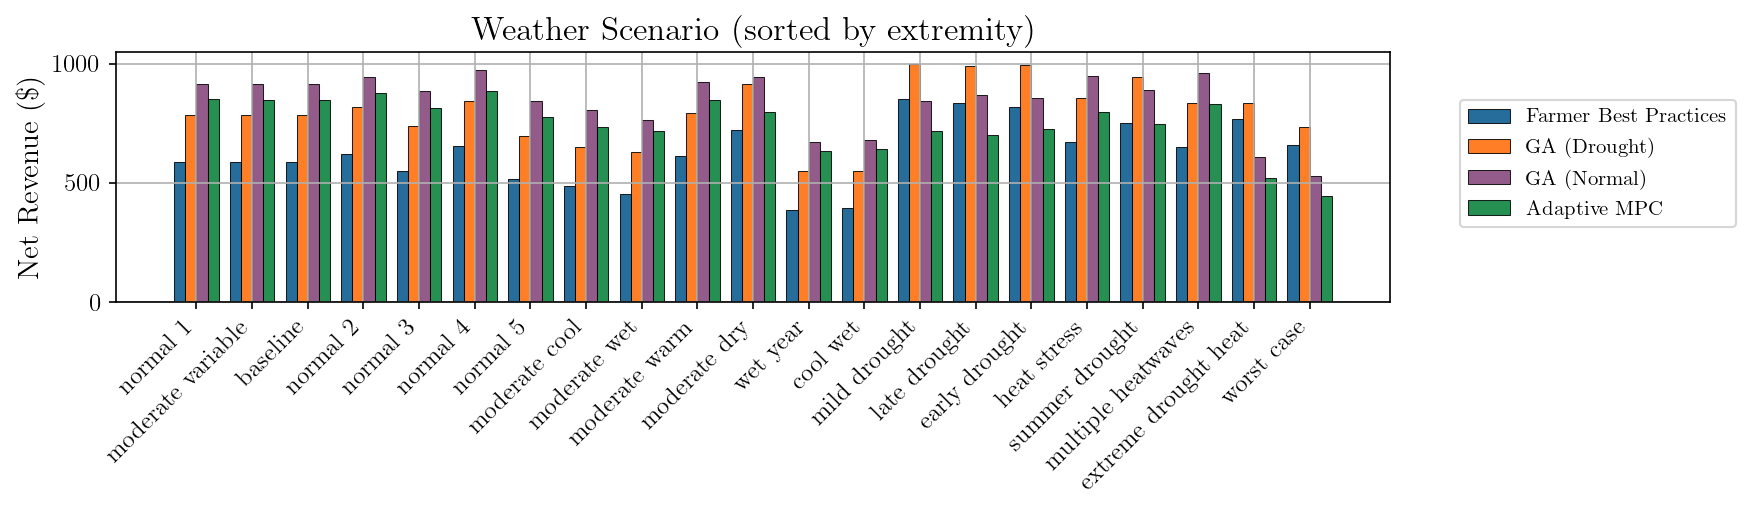
\includegraphics[width=\textwidth]{four_way_revenue_comparison.png}
\caption{Revenue comparison across all 21 weather scenarios, sorted by extremity index. Farmer best practices (blue), GA Drought (orange), GA Normal (purple), and Adaptive MPC (green). All optimization methods outperform farmer best practices. GA (Normal) dominates in normal/moderate conditions; GA (Drought) excels in drought scenarios.}
\label{fig:revenue-comparison}
\end{figure}

%------------------------------------%
% PERFORMANCE BY WEATHER TYPE
%------------------------------------%
\subsection{Performance by weather type}\label{subsec:weather-type-analysis}

To better understand when each strategy excels, we categorize scenarios by their extremity index and compute mean revenue within each category (Table~\ref{tab:category-results}).

\begin{table}[ht]
\centering
\begin{tabular}{|l|c|c|c|c|c|}
\hline
Weather Category & $n$ & Farmer & GA (Drought) & GA (Normal) & MPC \\
\hline\hline
Normal   (ext $<$ 0.5) & 7 & 586 & 778 & 913 & 842 \\
Moderate (0.5--1.5)    & 7 & 558 & 726 & 804 & 726 \\
Extreme  (ext $>$ 1.5) & 7 & 736 & 884 & 808 & 680 \\
\hline
\end{tabular}
\caption{Mean revenue (\$/acre) by weather category based on extremity index. Each GA strategy excels in conditions matching its optimization assumptions.}
\label{tab:category-results}
\end{table}

The results are straightforward: each GA strategy performs best when conditions match its optimization assumptions. GA (Normal) outperforms all other strategies in normal conditions by \$71/acre over MPC and \$135/acre over GA (Drought). In extreme conditions (primarily drought scenarios), GA (Drought) dominates with \$884/acre, outperforming GA (Normal) by \$76/acre. This is unsurprising---a strategy optimized for drought should excel in drought conditions.

MPC consistently underperforms the GA strategy appropriate for each condition. In normal conditions, MPC trails GA (Normal) by \$71/acre; in extreme conditions, MPC trails GA (Drought) by \$204/acre. MPC's adaptive behavior does not compensate for the GA's ability to pre-optimize for specific conditions. Figure~\ref{fig:by-category} illustrates this pattern.

\begin{figure}[ht]
\centering
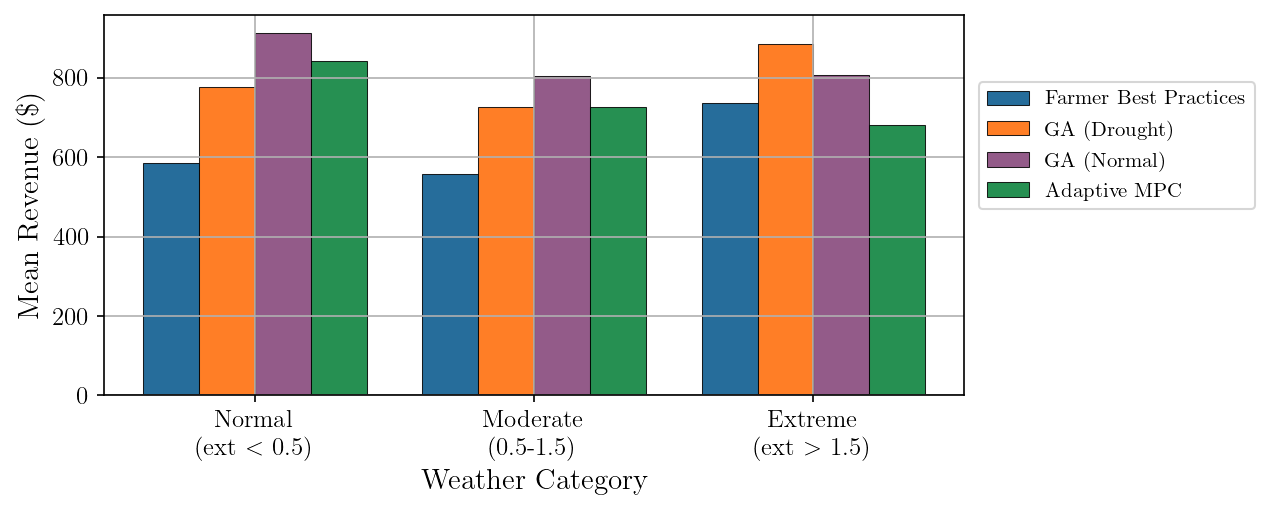
\includegraphics[width=\textwidth]{four_way_by_category.png}
\caption{Mean revenue by weather category. GA (Normal) (purple) dominates in normal and moderate conditions, while GA (Drought) (orange) excels in extreme conditions. MPC (green) underperforms the appropriate GA strategy in each category. All optimization methods outperform farmer best practices (blue).}
\label{fig:by-category}
\end{figure}

As a sanity check on our crop model, we compare the simulated farmer best practices revenue against real-world estimates. Current Iowa corn yields average approximately 225 bushels per acre \cite{robinson2025usda_crop_report_2025} at prices near \$4 per bushel \cite{usda2026iowa_daily_cash_grain_bids}. Variable costs for irrigation and fertilizer are approximately \$220 per acre \cite{swanson2025high_production_cost_series3}, yielding estimated net revenue of roughly \$680/acre under favorable conditions. Our simulated farmer best practices achieves a mean of \$626/acre across the weather scenario ensemble---within 8\% of this estimate, suggesting reasonable model calibration.


%------------------------------------%
% VARIANCE AND RISK
%------------------------------------%
\subsection{Variance and risk analysis}\label{subsec:risk}

The coefficient of variation (CV), defined as the ratio of standard deviation to mean, provides a normalized measure of consistency:
\begin{equation}
\text{CV} = \frac{\sigma}{\mu} \times 100\%
\label{eqn:cv}
\end{equation}

As shown in Table~\ref{tab:main-results}, GA (Normal) achieves the lowest CV (14.7\%), followed by MPC (15.4\%), GA (Drought) (16.6\%), and farmer best practices (21.6\%). MPC achieves the lowest absolute standard deviation (\$115 vs \$124 for GA Normal), but this does not compensate for its lower mean revenue.

The risk-return characteristics differ across strategies. GA (Drought) achieves the highest maximum revenue (\$997/acre in mild drought) but also experiences larger swings: its revenue ranges from \$550 to \$997, a spread of \$447. GA (Normal) achieves the highest mean (\$842/acre) with a similar range (\$527--\$973). MPC's range is slightly tighter at \$441 (\$445--\$886), with the lowest maximum.

For risk-averse decision-makers, the GA strategies provide better downside protection than MPC. Consider a farmer who must meet fixed costs of \$600/acre:
\begin{itemize}
\item GA (Drought) falls below this threshold in 2 scenarios (wet year and cool wet)
\item GA (Normal) falls below in 3 scenarios (wet year, cool wet, and worst case)
\item MPC falls below in 6 scenarios (the same three plus extreme drought heat, mild drought, and late drought)
\end{itemize}

Figure~\ref{fig:boxplot} shows the revenue distribution for each strategy as a box plot. GA (Normal) has the highest median and mean (red diamond). MPC has a tighter interquartile range, but this consistency comes at the cost of lower overall performance.

\begin{figure}[ht]
\centering
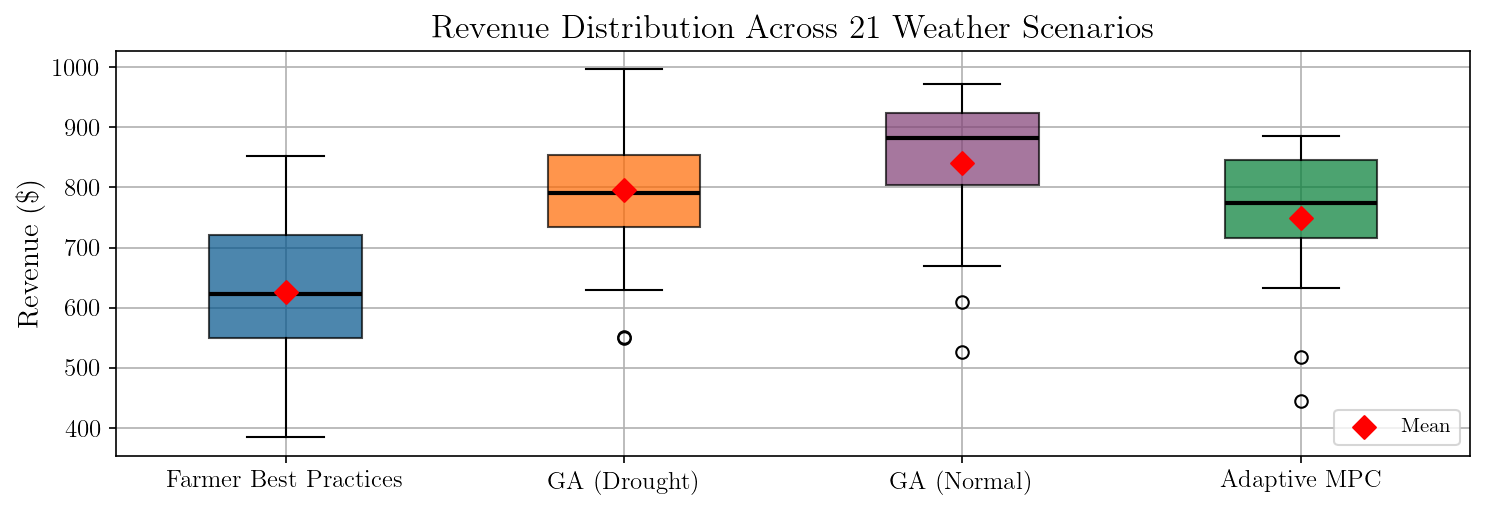
\includegraphics[width=\textwidth]{four_way_revenue_boxplot.png}
\caption{Revenue distribution across 21 weather scenarios. Box plots show median (black line), interquartile range (box), and full range (whiskers). Red diamonds indicate means. GA (Normal) achieves the highest mean revenue.}
\label{fig:boxplot}
\end{figure}

Figure~\ref{fig:cv-comparison} directly compares the coefficient of variation for each strategy. GA (Normal) achieves the lowest CV (14.7\%), followed by MPC (15.4\%), GA (Drought) (16.6\%), and farmer best practices (21.6\%). All optimization methods reduce relative variability compared to farmer best practices.

\begin{figure}[ht]
\centering
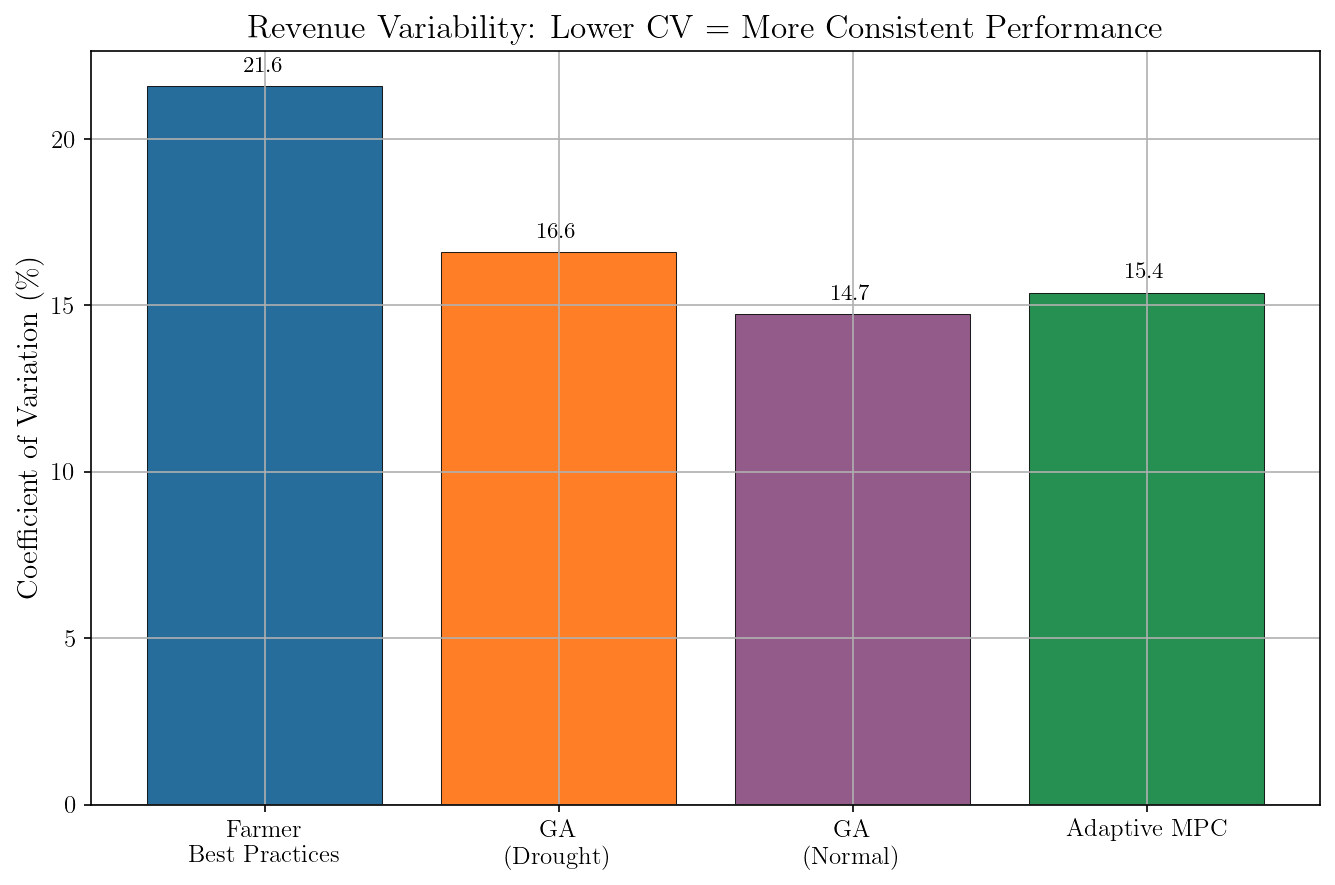
\includegraphics[width=0.7\textwidth]{four_way_cv_comparison.png}
\caption{Coefficient of variation (CV) comparison. Lower CV indicates more consistent relative performance. GA (Normal) achieves the lowest CV (14.7\%), followed by MPC (15.4\%), GA (Drought) (16.6\%), and farmer best practices (21.6\%).}
\label{fig:cv-comparison}
\end{figure}

%------------------------------------%
% RESOURCE ADAPTATION
%------------------------------------%
\subsection{Resource usage patterns}\label{subsec:resource-patterns}

MPC does adapt its resource usage across scenarios. While both GA strategies apply the same total irrigation regardless of conditions---GA (Drought) applies approximately 10 inches per season and GA (Normal) applies approximately 4 inches---MPC irrigation varies from 3.9 inches (wettest scenario) to 6.3 inches (driest scenario). However, this adaptation does not translate to better revenue outcomes.

The three fixed strategies differ substantially in their fertilizer application patterns. GA (Drought) applies fertilizer infrequently in large doses (77 lbs every 33 days), while GA (Normal) applies smaller, more frequent doses (30 lbs every 9 days). Farmer best practices use monthly applications of 90 lbs. MPC adapts its fertilizer usage based on observed plant state and weather.

This resource usage pattern explains the performance differences: GA (Normal)'s frequent, small fertilizer applications work well when water is available to transport nutrients, but become ineffective when precipitation is reduced. GA (Drought)'s infrequent, heavy irrigation applications are better suited to drought conditions. MPC's adaptive behavior cannot match the performance of a GA strategy pre-optimized for the actual conditions.

\textbf{Resource efficiency perspective.} While MPC does not achieve the highest revenue, it offers a different value proposition: achieving reasonable returns with substantially lower resource consumption. MPC outperforms farmer best practices in 15 of 21 scenarios while using dramatically less water and fertilizer---MPC applies only 1.3--2.0 inches of irrigation per season compared to 18 inches for farmer best practices and 15 inches for GA (Drought). Similarly, MPC uses 216--307 lbs of fertilizer compared to 450 lbs for farmer best practices. From a sustainability standpoint, MPC's resource efficiency may be valuable in contexts where environmental impact or input costs are prioritized over maximum yield.

%======================================================================================%
% DISCUSSION
%======================================================================================%
\section{Discussion}\label{sec:discussion}

%------------------------------------%
% INTERPRETATION
%------------------------------------%
\subsection{Interpretation of results}\label{subsec:interpretation}

Our results do not support the hypothesis that adaptive MPC can outperform fixed GA strategies. This section discusses why our hypothesis was incorrect and what practical conclusions can be drawn.

\textbf{Why MPC underperforms.} We hypothesized that MPC's ability to adapt to observed conditions would allow it to outperform strategies optimized for specific weather assumptions. This hypothesis was incorrect. The GA strategies, despite being ``fixed,'' are optimized for their target conditions over the entire growing season. MPC re-optimizes daily but only sees 9 days ahead (the planning horizon). This limited foresight prevents MPC from making the long-term resource allocation decisions that the GA can pre-compute. In agricultural systems with slow dynamics---where nutrient absorption takes days to weeks---the GA's full-season optimization horizon appears more valuable than MPC's adaptive but myopic decision-making.

Notably, the 9-day horizon was selected by Bayesian optimization as the best-performing choice within our computationally tractable search space (3--14 days). This suggests the limitation is not simply computational: even with the ``optimal'' horizon length, MPC underperforms. The more fundamental issue may be the mismatch between MPC's daily decision-making timescale and the crop's multi-week physiological response times. The delayed absorption effects modeled via FIR convolution (with time constants of 30--300 hours) mean that today's decisions primarily affect plant state 1--2 weeks later. By the time MPC observes the consequences of its actions, much of its planning horizon has already elapsed.

\textbf{When to use which GA strategy.} The practical conclusion is straightforward: choose the GA strategy optimized for expected conditions. If normal weather is anticipated, use GA (Normal); if drought is anticipated, use GA (Drought). The GA (Normal) strategy achieves \$913/acre mean revenue in normal conditions, while GA (Drought) achieves \$884/acre in extreme conditions. Each strategy is designed for specific conditions and performs best when those conditions occur.

\textbf{The limited value of adaptation.} MPC does adapt its resource usage---irrigation varies from 3.9 to 6.3 inches across scenarios---but this adaptation does not translate to better outcomes. The GA strategies apply fixed amounts regardless of conditions yet still outperform. This suggests that for seasonal agricultural planning, knowing the expected conditions and optimizing accordingly is more valuable than responding to observed conditions.

\textbf{Comparing the GA strategies.} The drought-optimized GA outperforms the normal-optimized GA only in drought scenarios. This is unsurprising given their design. The more interesting finding is that GA (Normal) achieves the highest mean revenue overall (\$842 vs \$796 for GA Drought), suggesting that optimizing for normal conditions is the better default choice unless drought is specifically anticipated.

%------------------------------------%
% COMPUTATIONAL CONSIDERATIONS
%------------------------------------%
\subsection{Computational considerations}\label{subsec:computational}

Several design choices were driven by computational tractability. First, we use a two-tier temporal scheme: plant dynamics are simulated at hourly resolution (matching the crop model's physiological timescales), but MPC decisions are made daily. This daily decision scale is both computationally necessary---solving 121 daily optimizations is tractable, while 2,900 hourly optimizations would be prohibitive---and practically realistic, as farmers cannot adjust irrigation and fertilization hourly. Second, the planning horizon is constrained to 3--14 days; longer horizons would increase the CFTOC problem size and solver time. Third, we use Python-based tools (Pyomo for problem formulation, IPOPT for solving) which prioritize flexibility over raw speed. A production implementation using compiled solvers (e.g., custom C++ code or MATLAB's \texttt{fmincon}) could potentially handle longer horizons, though our results suggest the fundamental limitation is structural rather than computational.

That said, each CFTOC solve requires approximately 0.5--1.0 seconds on a modern workstation using IPOPT. Over a 121-day growing season with daily re-optimization, total computation time is approximately 1--2 minutes. The Bayesian optimization for parameter tuning requires 100 trials, each involving multiple full-season MPC simulations. Total tuning time is approximately 2--4 hours, but this is a one-time offline computation. Once parameters are tuned, MPC operates with minimal computational burden.

%------------------------------------%
% LIMITATIONS
%------------------------------------%
\subsection{Limitations and extensions}\label{subsec:limitations}

Several limitations suggest directions for future work:

\textbf{Perfect forecast assumption.} Our MPC formulation assumes perfect weather forecasts over the planning horizon. In practice, forecast accuracy degrades with lead time. Incorporating forecast uncertainty through stochastic MPC or robust optimization would improve real-world applicability.

\textbf{Single-point model.} The crop model represents a single plant without spatial heterogeneity. Field-scale implementation would require accounting for spatial variation in soil properties, drainage, and microclimate.

\textbf{Simplified economics.} Our cost function uses constant economic weights. In practice, crop prices fluctuate seasonally, and input costs may have nonlinear components (e.g., volume discounts).

\textbf{Soil moisture dynamics.} The current model treats irrigation as directly available water without explicitly modeling soil moisture content. A more realistic extension would incorporate soil water balance dynamics, where leaf area expansion depends on soil water availability rather than irrigation input directly. This would enable modeling of drought stress accumulation, soil type effects on water retention, and the lag between irrigation events and plant-available water---factors that become increasingly important under variable weather conditions.


%======================================================================================%
% CONCLUSION
%======================================================================================%
\section{Conclusion}\label{sec:conclusion}

This paper tested whether adaptive Model Predictive Control could outperform fixed genetic algorithm strategies for irrigation and fertilizer scheduling under weather uncertainty. We developed an MPC framework with Bayesian-optimized parameters and compared it against farmer best practices and two GA strategies (optimized for normal and drought conditions) across 21 stochastic weather scenarios.

Our hypotheses and findings are:

\begin{enumerate}
\item \textbf{Hypothesis 1 (supported):} All optimization-based methods outperform farmer best practices. GA (Normal) achieves a mean advantage of \$215/acre, GA (Drought) achieves \$170/acre, and MPC achieves \$123/acre.

\item \textbf{Hypothesis 2 (not supported):} MPC does not outperform the GA strategies. GA (Normal) outperforms MPC in all 21 scenarios. MPC's adaptive behavior cannot compensate for the GA's ability to pre-optimize for specific conditions.

\item \textbf{Hypothesis 3 (partially supported, but trivially so):} GA (Drought) outperforms GA (Normal) only in drought scenarios---an unsurprising result given it was optimized for those conditions. GA (Normal) achieves the highest overall mean revenue (\$842/acre vs \$796/acre for GA Drought).
\end{enumerate}

The practical conclusion is straightforward: for seasonal agricultural planning, pre-optimization for expected conditions outperforms adaptive control. If normal weather is expected, use GA (Normal); if drought is expected, use GA (Drought). MPC's daily adaptation cannot substitute for the GA's full-season optimization horizon. However, MPC offers a sustainability advantage worth noting: it achieves competitive returns (outperforming farmer best practices in 15 of 21 scenarios) while using dramatically less water (1.3--2.0 inches vs.\ 15--18 inches for other strategies) and fertilizer (216--307 lbs vs.\ 450 lbs for farmer best practices). For operations prioritizing environmental impact or input cost reduction, MPC may be the preferred choice despite lower peak revenue.

Why did MPC underperform? Agricultural systems have slow dynamics---nutrient absorption takes days to weeks. MPC's 9-day planning horizon limits its ability to make the long-term resource allocation decisions that the GA can pre-compute over the entire growing season. In systems where the relevant timescales exceed the controller's horizon, pre-optimization may generally outperform adaptive control.

Future work could explore longer MPC horizons, stochastic MPC that accounts for weather uncertainty, or hybrid strategies. Field validation would determine whether these results generalize beyond the simulation environment.

%======================================================================================%
% ACKNOWLEDGEMENTS
%======================================================================================%
\section*{Acknowledgements}

This work has been partially supported by the UC Berkeley College of Engineering and the USDA AI Institute for Next Generation Food Systems (AIFS), USDA award number 2020-67021-32855.

%======================================================================================%
% DECLARATIONS
%======================================================================================%
\section*{Declarations}

\noindent\textbf{Competing Interests}
\noindent The authors declare that they have no known competing financial interests or personal relationships that could have appeared to influence the work reported in this paper. \\

\noindent\textbf{Code availability}
\noindent The source code used for this study is archived on Zenodo at \url{https://doi.org/10.5281/zenodo.18204023}. \\

\noindent\textbf{Declaration of generative AI and AI-assisted technologies in the manuscript preparation process}
\noindent During the preparation of this work the authors used ChatGPT and Claude Code in order to generate some portions of the code base, though no underlying theory, and refine the original drafts of the paper. After using this tool/service, the authors reviewed and edited the content as needed and take full responsibility for the content of the published article.

%======================================================================================%
% BIBLIOGRAPHY
%======================================================================================%
\bibliographystyle{elsarticle-num} 
\bibliography{bibliography}

\end{document}
